This section should provide the theoretical background and the foundation of the conducted study.
Therefore, this section is structured as follows: 
first, related work of stock market prediction will be presented in \cref{s:background-stockmarketprediction};
second, an introduction into option mining will be given in \cref{s:background-optionmining};
and third, the market of social networks will be examined in \cref{s:background-socialnetworks}.

\section{Stock Market Prediction} 
\label{s:background-stockmarketprediction}

\citeauthor{Bollen2011a} noted that many researches assumed that the stock market is based on the random walk theory and the \ac{EMH}.
First, the \ac{EMH} suggests that the price of a security is reflected by all information available \cite{fama1965behavior, schumaker2009textual}.
Furthermore, the \ac{EMH} can be split into three forms: the Weak, the Semi-Strong and the Strong.

\begin{itemize}
    %\itemsep0em
    \item
        In Weak \ac{EMH} only historical information is incorporated in the current price \cite{schumaker2009textual}.

    \item
        In Semi-Strong \ac{EMH} uses historical and also currently available public information in the current price \cite{schumaker2009textual}.

    \item
        In Strong \ac{EMH} the Semi-Strong model is enhanced with currently available private information such as insider information in the share price \cite{schumaker2009textual}.
\end{itemize}

Therefore, the \ac{EMH} assumes that stock market prices are driven by new information such as news and will less depend on the current price or historical prices.
As news are unpredictable the stock market prices will follow a random walk pattern \cite{Bollen2011a}.

But \citeauthor{Bollen2011a} stated also that stock prices aren't following the random walk pattern completely and can therefore predicted in some way.
They stated that information available online may act as early indicators for changes.
This include the Google search queries which provide an early indicator for disease infections (see \url{https://www.google.org/flutrends/}) \cite{Bollen2011a}.

These effects can be also applied to the stock markets: not just news influences the stock market but also the public opinion and mood.
Previously large surveys have been conducted to gather the public mood of a representative sample.
This was very time consuming and expensive.
But in the last ten years a significant progress has been made in sentiment tracking techniques.
Therefore the sentiments can be extracted from news and blogs
\cite{Bollen2011a}.


\section{Option Mining} 
\label{s:background-optionmining}

Option mining is defined as extracting opinions from unstructured data using natural language processing techniques \cite[page 411]{Liu2007}.

According to Pang and Lee the two terms \emph{option mining} and \emph{sentiment analysis} are mere synonyms within this field of study \cite{Pang2008c}.
Therefore, this study will use the terms interchangeably.

There are several types of option mining available:

\begin{enumerate}
	\item 
	Sentiment classification: 
	This task is performed on a document level and classifies the text as positive or negative. 
	No further analysis is made what people may like or dislike 
	\cite[page 411]{Liu2007}.
	
	\item 
	Feature-based opinion mining and summarization: 
	This task dives deep into the text and analyzes the sentences on it's own.
	Furthermore, it discovers the opinions on objects which are liked or disliked.
	An object may be a product, service, topic or organization. 
	For example in an product review it detects the product features which have been described 
	\cite[page 412]{Liu2007}.
	
	\item
	Comparative sentence and relation mining:
	In this type of task product features are compared to the same or similar feature of another product.
	For example comparing two cameras: "the battery life of camera A is much shorter than that of camera B" 
	\cite[page 412]{Liu2007}. 
\end{enumerate}

This study will focus on short documents with given keywords in it. 
Therefore, we assume that the documents describing our targeted topic.
As a result the study will focus on sentiment classification.

Sentiment classification has some similarities with topic-based text classification, which classifies the topic of documents into predefined topic classes, for example sports, science or politics.
In topic based classification topic words are important, while they are unimportant for sentiment classification \cite[page 412f]{Liu2007}.

In the following an introduction into sentiment detection techniques will be given, including:

\begin{itemize}
    \item Text preprocessing (see \cref{ss:background-optionmining-textpreprocessing})
    \item Text Vectorization (see \cref{ss:background-optionmining-textvectorization})
    \item Machine Learning Algorithms (see \cref{ss:background-optionmining-machinelearningalgorithms})
\end{itemize}

For these sections the variable definitions of \autoref{tab:background-optionmining-variables} apply.

\begin{table}
	\begin{center}
		\begin{tabular}{l l}
			\textbf{Element} & \textbf{Description} \\ \hline
			$c$ & Specific document class \\
			$C$ & Document classes \\
			$d$ & Specific document \\
			$D$ & Documents \\
			$f_i$ & Specific feature \\
			$m$ & Count of features \\
			$n_i(d)$ & Count of features $i$ in document $d$ \\
			$P(x)$ & Probability of x \\
		\end{tabular}

        \caption{Variable definitions used in option mining}
        \label{tab:background-optionmining-variables}
	\end{center}
\end{table}

\subsection{Text Preprocessing}
\label{ss:background-optionmining-textpreprocessing}

%pre processing
%stop word
%stemming

\subsection{Text Vectorization}
\label{ss:background-optionmining-textvectorization}

%bag of words 
%uni-grams
%bi-grams
%tri-grams

%term frequency (tf)
%inverse document frequency (idf)

%TF-IDF: \cite{Bafna2016}

\subsection{Machine Learning Algorithms}
\label{ss:background-optionmining-machinelearningalgorithms}

\citeauthor{Pang2002} performed a study which analyzed several machine learning algorithms and their suitability with sentiment classification.
These three algorithms have shown a good performance in text categorization studies and therefore they tried to apply these algorithms to sentiment classification \cite{Pang2002}.

\begin{description}
	\item[Naive Bayes.] 
    The \ac{NB} algorithm calculates the probabilities that a document $d$ belong to a class $c$.
	Furthermore, it implies that all classes are independent to each other, which does not hold true very often in a real world scenario.
	In sentiment classification tasks there are two classes available: positive and negative.
	Therefore the text is classified as class $c$ where $c* = arg max_c P(c | d)$.
	The general Bayes classifier can be seen in \autoref{eq:background-optionmining-machinelearningalgorithms-bayes} \cite{Pang2002}.
	
	\begin{equation}
		P_{NB}(c|d) = \frac{P(c) (\prod_{i=1}^{m} P(f_i|c)^{n_i(d)}) }{P(d)}
		\label{eq:background-optionmining-machinelearningalgorithms-bayes}
	\end{equation}
	
	Despite the fact that the Naive Bayes algorithm is very simple and the assumption of independent classes does not hold true in a real world scenario it performs surprisingly well \cite{Pang2002}.
	
	\item[Maximum Entropy Classification.]
  The \ac{ME} Classification succeeded in a number of language processing applications.
  The exponential form of the Maximum Entropy Classifier can be seen in \autoref{eq:background-optionmining-machinelearningalgorithms-maximumentropy} \cite{Pang2002}.
  
  \begin{equation}
    P_{ME}(c|d) = \frac{1}{Z(d)} exp \left( \sum_i^m \lambda_{i,c}F_{i,c}(d,c) \right)
    \label{eq:background-optionmining-machinelearningalgorithms-maximumentropy}
  \end{equation}
  
  Whereas $Z(d)$ is a normalization function as depicted in \autoref{eq:background-optionmining-machinelearningalgorithms-maximumentropy_Zd} \cite{Nigam1999} and $F_{i,c}(d,c)$ is a feature/class function for feature $f_i$ and class $c$ which is defined in \autoref{eq:background-optionmining-machinelearningalgorithms-maximumentropy_fic}.

  \begin{equation}
    Z(d) = \sum_c exp(\sum_i \lambda_{i,c} F_{i,c}(d,c))
      \label{eq:background-optionmining-machinelearningalgorithms-maximumentropy_Zd}
  \end{equation}

  \begin{equation}
  F_{i,c}(d,c') = 
    \begin{cases}
      1, & n_i(d) > 0 \text{ and } c' = c \\
      0  & \text{otherwise}
    \end{cases}
	\label{eq:background-optionmining-machinelearningalgorithms-maximumentropy_fic}
  \end{equation}

  $\lambda_{i,c}$ are feature weight parameters. A larger value of that parameter means that feature $f_i$ is considered as strong indicator for class $c$.
  The values for $\lambda_{i,c}$ are set in a way that the entropy of the training data set is maximized \cite{Pang2002}.
  	
	\item[Support Vector Machine.]
   \ac{SVM} are large-margin classifiers in contrast to the probabilistic Naive Bayes and Maximum Entropy.
   That means that in the two-category case (positive or negative) the training procedure looking for a hyperplane which maximizes the margin between the two groups \cite{Pang2002}.
   This scenario is depicted in \autoref{fig:background-optionmining-machinelearningalgorithms-svm} \cite[p. 275]{Cortes1995}.
      
   \begin{figure}[ht]
    \centering
    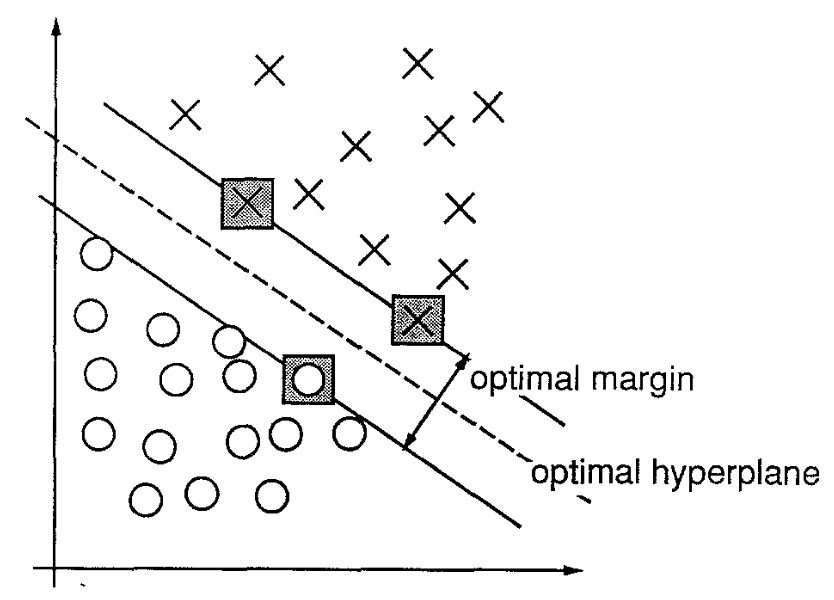
\includegraphics[width=.7\textwidth]{images/svm.png}
    \caption{An example of a two-category case, from \cite[p. 275]{Cortes1995}}
    \label{fig:background-optionmining-machinelearningalgorithms-svm}
  \end{figure}
	
\end{description}

\section{Social networks/microblogging services}
\label{s:background-socialnetworks}

In the last years many social networks started and many of them disappeared again.
There are several types of social networks available today: some of them are built on videos others on pictures and some of them mostly on text.
Those which are built on text are more easy to analyze and searchable for researchers worldwide.
But there are some constants in this field: Twitter, to identify one of them.
Twitter has become a valuable source of opinions, data and information for various researches \cite{Barbosa2010}.

Messages on Twitter are called tweets and are limited in length (140 for tweets before November 7th 2017; 280 characters since then, at least for english tweets \cite{Rosen2017}) users have to concentrate on a specific topic precisely.
Therefore, Twitter is the perfect source of the public opinion as users discussing anything on Twitter \cite{Pagolu2016a}.

As a result the fields in which researches have used data from Twitter ranging from public opinions for politicans and polls (see \cite{Oconnor2010a,Patodkar2016a}) to the stock market and the prediction of stock prices and other factors (see \cite{Bollen2011a,Mittal2012a,Nguyen2015a,Pagolu2016a,Zhang2011a}).

% On the other hand keywords like cloud, machine learning and artificial intelligence are everywhere. 
% Amazon, Facebook, Google, IBM and Microsoft and other big players of the industry are making massive progress in these fields.